\documentclass[11pt,letterpaper,twocolumn]{article}

\usepackage[utf8]{inputenc}
\usepackage[spanish]{babel}
\usepackage{float}
\usepackage{xcolor}
\usepackage{verbatim}
\usepackage{mwe}
\usepackage{charter}
\usepackage{afterpage}
\usepackage{amsmath}
\usepackage{appendix}
\usepackage{ragged2e}
\usepackage{array}
\usepackage{etoolbox}
\usepackage{fancyhdr}
\usepackage{booktabs}
\usepackage{arydshln}
\usepackage[justification=justified,singlelinecheck=false,labelfont=bf,format=plain]{caption}
\usepackage[justification=justified,singlelinecheck=false,labelfont=bf,format=plain]{subcaption}
\usepackage{enumitem}
\usepackage[bottom=2.5cm,top=2.0cm,left=2.0cm,right=2.0cm]{geometry}
\usepackage{graphicx}
\usepackage{indentfirst}
\usepackage{mathtools}
\usepackage{multirow}
\usepackage{pdfpages}

\usepackage{subfiles}
\usepackage[compact]{titlesec}
\usepackage{blindtext}
\usepackage{stfloats}
\usepackage{lipsum} 


\renewcommand{\familydefault}{\rmdefault}

\newcommand\blankpage{
    \null
    \thispagestyle{empty}
    \addtocounter{page}{0}
    \newpage}

\newcolumntype{L}[1]{>{\raggedright\let\newline\\arraybackslash\hspace{0pt}}m{#1}}
\newcolumntype{C}[1]{>{\centering\let\newline\\arraybackslash\hspace{0pt}}m{#1}}
\newcolumntype{R}[1]{>{\raggedleft\let\newline\\arraybackslash\hspace{0pt}}m{#1}}

    \setlist[itemize,1]{label=$\bullet$}
    \setlist[itemize,2]{label=$\circ$}
    \setlist[itemize,3]{label=$-$}
    \setlist{nosep}

\setlength{\columnsep}{30pt}

\titlelabel{\thetitle.\quad}

\pagestyle{fancy}
\fancyhf{}
      
\fancyfoot{}
\fancyfoot[C]{\thepage} % page
\renewcommand{\headrulewidth}{0mm} % headrule width
\renewcommand{\footrulewidth}{0mm} % footrule width

\makeatletter
\patchcmd{\headrule}{\hrule}{\color{black}\hrule}{}{} % headrule
\patchcmd{\footrule}{\hrule}{\color{black}\hrule}{}{} % footrule
\makeatother

\definecolor{blueM}{cmyk}{1.0,0.49,0.0,0.47}

%%%%%%%%%%%%%%%%%%%%%%%%%%%%%%%%%%%%%%%%%%%%%%%%%%%%%%%%%%%%%%%%%%%%%%%%%%%%%%%%%%%%%%%%%%%%%%%%%%%%%%%%%%%%%%%%%%%%%%%%%%%%%%%%%%%%%%%%%%%%%%%%%%%%%%%%%%%%%%%%%%%%%%%%%%%%%%%%%%%%%%%%%%%%%%%%%%%%%%%%%%%%%%
%%%%%%%%%%%%%%%%%%%%%%%%%%%%%%%%%%%%%%%%%%%%%%%%%%%%%%%%%%%%%%%%%%%%%%%%%%%%%%%%%%%%%%%%%%%%%%%%%%%%%%%
%%%%%%%%%%%%%%%%%%%%%%%%%%%%%%%%%%%%%%%%%%%%%%%%%%%%%%%%%%%%%%%%%%%%%%%%%%%%%%%%%%%%%%%%%%%%%%%%%
\title{Práctica 5. Ciclo de histéresis}
\author{Álvaro Martín Romero \\
Manuel Pérez Luna\\
Roberto Rodríguez Vaz}
\begin{document}
\twocolumn[\begin{@twocolumnfalse}
\maketitle
\small


\centerline{\rule{0.95\textwidth}{0.4pt}}

\begin{center}
    
    \begin{minipage}{0.9\textwidth}
        % RESUMEN
        \noindent \textbf{Resumen:} La histéresis es una propiedad magnética de los materiales que se refiere a la tendencia de conservar el campo magnético debido a la ausencia del estímulo que lo ha generado. Para saber esta característica de algunos materiales, hallaremos el ciclo de histéresis de un núcleo de hierro macizo y laminado. 
    
        \vspace{4mm}
        % PALABRAS CLAVE
        \noindent \textbf{Palabras clave:} Campo magnético, histéresis, ausencia de estímulo
    
    \end{minipage}
    
\end{center}
\centerline{\rule{0.95\textwidth}{0.4pt}}
\vspace{15pt}
\end{@twocolumnfalse}]
%%%%%%%%%%%%%%%%%%%%%%%%%%%%%%%%%%%%%%%%%%%%%%%%%%%%%%%%%%%%
\section{Introducción}%
\label{}
El estímulo con el que será sometido los materiales es un campo magnético que le aplicamos. Debido a este campo magnético, los  ferromagnéticos (como el hierro) son materiales que son capaces de mostrar una magnetización permanente en ausencia de campo magnético. Esto es debido a la capacidad que tienen los dipolos para alinearse en regiones llamadas dominios
\subsection{Medida de la curva de histéresis}
La curva de histéresis es una gráfica donde se representa la intensidad del campo magnético con el campo $\vec{H}$ de forma que dispondremos de un núcleo de hierro donde se enrrolla una bobina que se le hace pasar una corriente  $I$, creando un campo magnético en el interior del metal. \\
\\
El campo $\vec{H}$ es aproximádamente uniforme y de módulo:
 \begin{equation}
	 \vec{H}=\frac{N}{L}I
\end{equation}
donde $N$ es el número de vueltas, $L$ es la longitud de la bobina e $I$ es la intensidad que recorre la bobina, medido experimentalmente esos datos podemos hallar $H$. \\
\\
Debemos tener en cuenta que, al magnetizar el metal, la curva que describe el campo magnético en función de $H$ es la primera curva de imanación, por tanto, no debemos de tomarla en cuenta para la histéresis. A partir de cierto valor disminuimos nuestra intensidad (y por ende $H$ ) hasta encontrarnos el punto $\left( -B_{max},-H_{max} \right) $, es decir, el punto simétricamente opuesto al máximo tomado anteriormente. 


\section{Resultados}%
\subsection{Núcleo macizo}%
\label{sec:}
Representamos la curva de histéresis:
\vfill
\hfill
\begin{figure}[H]
	\centering
	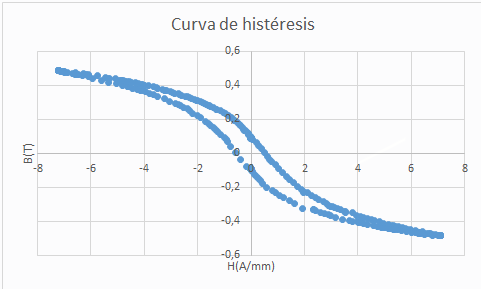
\includegraphics[width=0.5\textwidth]{imagen/mazico.png}
	\caption{Representación gráfica de la curva de histéresis de un núcleo mazico. Vemos como curiosidad como los datos han sido tomados con la corriente en signo contrario al que usamos normalmente para comparar curvas de histéresis.}
	\label{fig:imagen-macizo-png}
\end{figure}
El campo $\vec{B}_{rem}$ se define como el valor del campo magnético una vez hemos anulado el campo  $\vec{H}$. Por tanto, obtenemos dos valores,  $\vec{B}^+_{rem}$ y  $\vec{B}^-_{rem}$\\
\\
De la misma forma llamamos al campo $H_{coer}$ al campo  $H$ coecertivo , esto es, el valor de $H$ que hay que aplicar para anular el campo magnético $B$. Al igual que antes, hay dos puntos $\vec{H}^+_{coer}$ y  $\vec{H}^-_{coer}$\\
\\

De la gráfica podemos podemos obtener esos puntos  tomando el promedio de los resultados obtenidos para cada rama. Para ello interpolamos los datos obtenidos para los puntos que nos hacen falta. Los resultados son:

\begin{itemize}
	\item \textbf{$\vec{B}_{rem}$}
\begin{equation}	
	\boxed{\vec{B}^+_{rem}=0.08833865 T}
\end{equation}
\begin{equation}
	\boxed{\vec{B}^-_{rem}=-0.0942333 T}
\end{equation}

\item $\vec{H}_{coer}$
	 \begin{equation}
		 \boxed{\vec{H}^+_{coer}=0.5113362 \left( \frac{A}{mm} \right) }
	 \end{equation}
	 \begin{equation}
		 \boxed{\vec{H}^-_{coer}=-0.5684316 \left( \frac{A}{mm} \right) }
	 \end{equation}
\end{itemize}
Para el cálculo de la energía disipada necesitamos saber el área que encierra la curva de histéresis , para ello necesitamos integrar la función que sigue dicha curva, para obtener esta función representamos la curva de histéresis y añadimos una línea de tendencia del tipo polinómica , en concreto de grado 6. \\
\\
Para la rama de arriba:
\[
B(H)=-3\cdot 10^{-6}\cdot H^6 - 3\cdot 10^{-5}\cdot H^5 + 0.0003\cdot H^4 +\ldots .
\]
\[
	+ 0.0029\cdot H^3 -0.0092\cdot H^2-0.1395\cdot H+0.0885
.\] 
Para la rama de abajo:
\[
	B(H)=2\cdot 10^{-6}\cdot H^6 - 3\cdot 10^{-5}\cdot H^5 - 0.0002\cdot H^4+ \ldots	
.\] 
\[
	+ 0.003\cdot H^3 +0.0073\cdot H^2-0.405\cdot H+0.0876
.\] 
Integrando entre los límites de integración para el valor de $H_{max}$ y  $-H_{max}$ y sumando ambas integrales nos queda que:
\begin{equation}
	\boxed{U=0.87379}
\end{equation}

\section{Núcleo laminado}%
\label{se}
Representamos la curva de histéresis:
\begin{figure}[H]
	\centering
	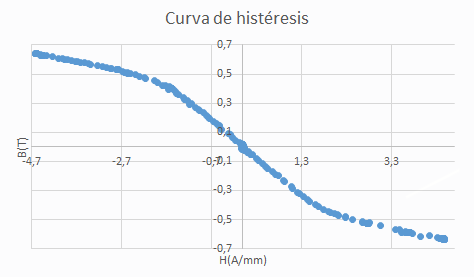
\includegraphics[width=0.5\textwidth]{imagen/laminado.png}
	\caption{Representación gráfica de la curva de histéresis para un núcleo laminado.}
	\label{fig:imagen-laminado-png}
\end{figure}
De la misma forma que antes, obetnemos los valores del campo magnético remanente y la intensidad $H$ coecertivo:

\begin{itemize}
	\item \textbf{$\vec{B}_{rem}$}
\begin{equation}	
	\boxed{\vec{B}^+_{rem}=0.008672242 T}
\end{equation}
\begin{equation}
	\boxed{\vec{B}^-_{rem}=-0.01670536 T}
\end{equation}

\item $\vec{H}_{coer}$
	 \begin{equation}
		 \boxed{\vec{H}^+_{coer}=0.015448399 \left( \frac{A}{mm} \right) }
	 \end{equation}
	 \begin{equation}
		 \boxed{\vec{H}^-_{coer}=-0.024159817 \left( \frac{A}{mm} \right) }
	 \end{equation}
\end{itemize}
Haremos lo mismo que hicimos anteriormente para hallar la energía, de forma que:\\
\\
Para la rama de arriba:
\[
B(H)=2\cdot 10^{-5}\cdot H^6  - 0.0003\cdot H^5 - 0.0006\cdot H^4 + \ldots .
\]
\[
	+ 0.0129\cdot H^3 +0.0032\cdot H^2-0.2741\cdot H+0.008
.\] 
Para la rama de abajo:
\[
	B(H)=3\cdot 10^{-6}\cdot H^6 - 0.0003\cdot H^5 - 0.0001\cdot H^4+ \ldots	
.\] 
\[
	+ 0.0119\cdot H^3 +0.0019\cdot H^2-0.2687\cdot H- 0.093
.\] 
Integrando entre los límites de integración para el valor de $H_{max}$ y  $-H_{max}$ y sumando ambas integrales nos queda que:
\begin{equation}
	\boxed{U=0.13971}
\end{equation}
\section{Conclusión}%
\label{secas}
\subsection{Definiciones}
\begin{itemize}

	\item Paramagnetismo: Las sustancias paramagnéticas son  átomos e iones que tienen en su capa más externa electrones desparejados, por lo que el momento del dipolo magnético de estos electrones no se ven cancelados. Esto hace que los átomos y los iones estén dotados de un momento dipolar magnético intrínseco sin la necesidad de un campo magnético externo. Sin embargo, si colocamos un material paramagnético en un campo externo, los espines paramagnéticos responden al campo magnético aplicado, por lo que se observa una significativa carga de magnetización debido a la orientación prioritaria de los momentos dipolares paralelas al campo magnético. La carga de este momento paramagnético es proporcional al campo externo aplicado, su susceptibilidad magnética es mayor que la de los diamagnéticos debido a la orientación de sus dipolos magnéticos (aunque experimentalmente esta orientación paralela no es tan perfecta ya que se ve influenciada por la temperatura). \\
\\


\item Diamagnetismo:  El diamagnetismo es una medida para indicar la capacidad de magnetizar un material, por lo que es una propiedad que poseen todos los materiales, aunque en algunos será más apreciable que en otros ya que las fuerzas  paramagnéticas y ferromagnéticas pueden hacer que se disipe. \\
	\\
El diamagnetismo aparece cuando existen átomos con pares de electrones en cada subcapa, es decir, con un momento del dipolo magnético nulo, e interactúan con un campo magnético externo apareciendo una pequeña alteración en el movimiento de la órbita de los electrones lo que genera  una pequeña magnetización. Como curiosidad, este campo magnético creado es antiparalelo al campo magnético externo y proporcional a la intensidad de este.\\
\\


\item Ferromagnetismo: El ferromagnetismo es una propiedad de grupo, que poseen los átomos o moléculas en un cristal sólido. Estos materiales poseen una interacción en grupo y están magnéticamente ordenados haciendo que estén siempre magnetizados por zonas. Un material ferromagnético desmagnetizado se divide por zonas con direcciones arbitrarias de magnetización que producen una magnetización neta nula. Pero, como estos materiales poseen una tremenda susceptibilidad magnética, con la interacción de un pequeño campo magnético se magnetizará ya que todos momentos magnéticos de cada región se orientará de forma paralela ampliando así el propio campo magnético. Debido a esta alta susceptibilidad ferromagnética, estos materiales pueden ser magnetizados hasta la saturación y mantener una carga magnética incluso cuando el campo es retirado.\\
\\
\end{itemize}
\section{Discusión de resultados}%
\label{sec}
Podemos observar que existen varias diferencias evidenciales en los resultados obtenidos en cada núcleo.\\
\\
En primer lugar vemos una gran diferencia en la curva de histéresis, para el caso del núcleo macizo esta curva es mucho más marcada, este resultado era de esperar ya que la curva de histéresis nos da la información de la tendencia del material a conservar la magnetización en ausencia del campo generador, por consiguiente, es lógico esperar que la capacidad para el núcleo macizo sea significativamente mayor al laminado.  Este resultado se hace aún más evidente al comparar las energías disipadas en ambos núcleos la cual es proporcional al área que encierra la curva de histéresis, donde el valor de núcleo macizo es 6,25 veces mayor que la del núcleo laminado.\\
\\
En segundo lugar podemos comparar los resultados del campo magnético remanente y del campo coercitivo. Cabe destacar que la coercitividad en los materiales ferromagnéticos nos indica la potencialidad de este para ser un imán permanente. Nuevamente, estos resultados ponen en evidencia lo comentado con anterioridad, tras aplicar la misma intensidad de campo magnético la magnetización remanente en el núcleo macizo es 6 veces mayor que para el laminado, y, como es de esperar, es necesaria una mayor intensidad de campo magnético (24 veces mayor) para poder desmagnetizar el núcleo macizo. \\
\\
En resumen, hemos conseguido poner en evidencia las capacidades ferromagnéticas de los distintos materiales de forma muy satisfactoria viendo como reaccionan al campo magnético.

\end{document}
